\subsubsection{K-Greedy Approach}\label{k-Greedy Approach}
~

\begin{figure}[htb]
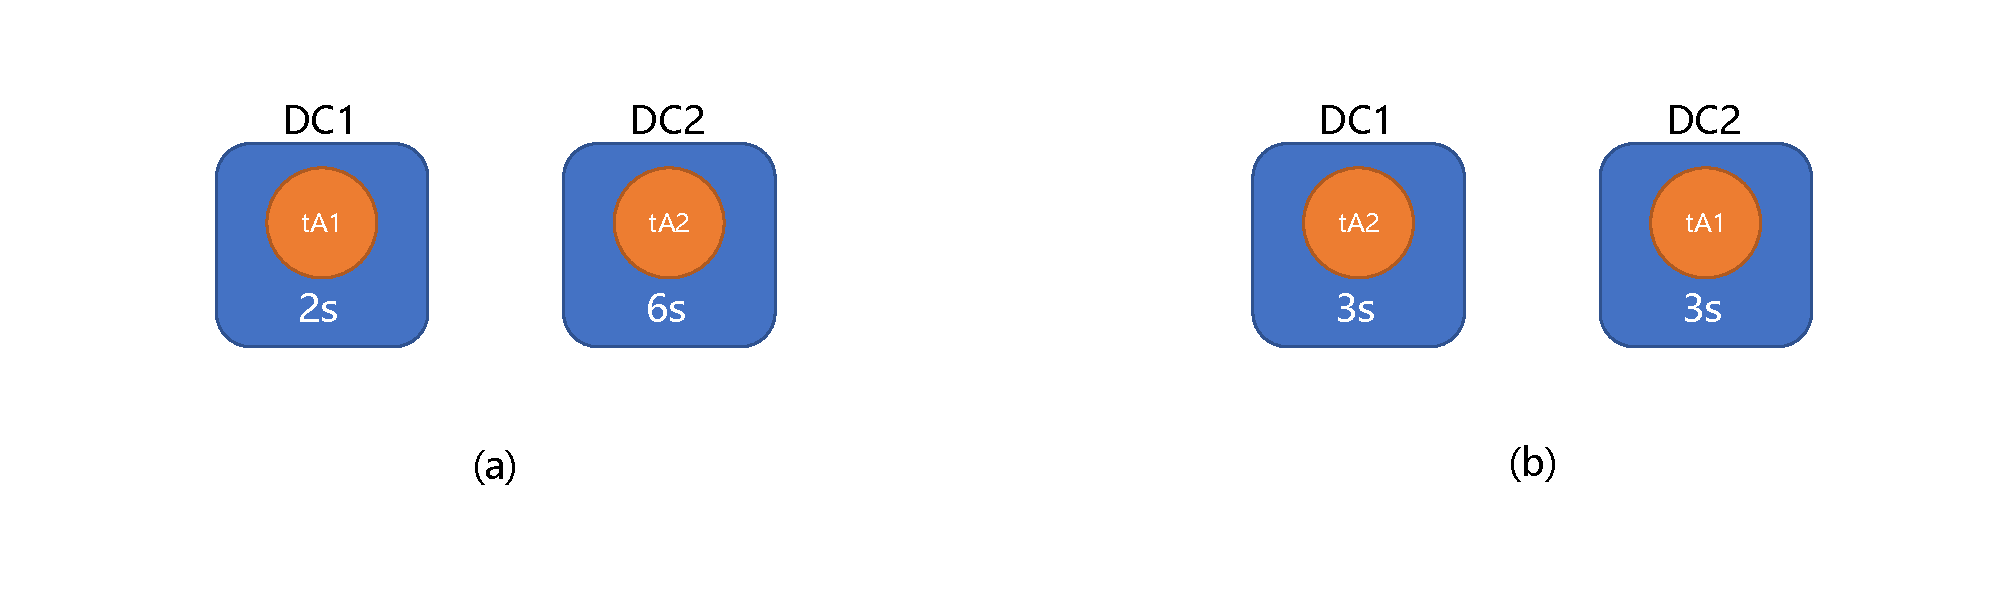
\includegraphics[width=1\textwidth]{figure/fig-greedy_eg.pdf}
\centering
\caption{Two possible assignments of tasks} \label{greedy_eg}
\end{figure}

When invoking Greedy Approach, we only consider about the very first task. And this may worsen the data transferring time of other tasks. This is better illustrated with example Fig. \ref{greedy_eg}. Greedy Approach first considers tA1 then tA2 and results in case (a). However, it is obvious that case (b) is better in both sum completion time and maximal completion time. Here, we introduce a randomized greedy approach, which is called K-Greedy Approach.

\textbf{Procedure}.
K-Greedy Approach randomly generate $k\sim U(0,2)$ for every task. Every time we compute an assignment with shortest data transferring time, we check whether $k$ is 0. If $k>0$, we simply skip this assignment and decrease $k$ by 1.

        % \begin{minipage}[t]{0.8\textwidth}
        %       \begin{algorithm}[H]
        %           %\LinesNumbered
        %           \KwIn{$x$, $y$}
        %           \KwOut{$sign$}
        %           \BlankLine
        %           \caption{$K-Greedy$} \label{Greedy_algo}

        %           $computes\ all\ possible\ assignments\ and\ put\ into\ priority\ queue$\;
        %           $randomly\ generate \ array\ K$\;
        %           $cnt \leftarrow 0$\;
        %           \While{$cnt < task\  number$}
        %           {
        %               $find\ assignment\ with\ shortest\ transferring\ time$\;
        %               $task \leftarrow assignment.task$\;
        %               \If{$K[task]>0 $ }
        %               {
        %                   $K[task]\leftarrow K[task]-1$\;
        %               }
        %               \ElseIf{$task \ is\ not\ assigned$}
        %               {
        %                   $bring\ this\ assignment\ into\ effect$\;
        %                   $cnt\leftarrow cnt+1$\;
        %               }
        %           }
        %       \end{algorithm}
        %   \end{minipage}

\textbf{Time Complexity}.
It may need k more iterations. Thus, time complexity is $O(km\log (|J|m))$.

K-Greedy Approach is able to yield case (b) in Fig. \ref{greedy_eg}. However, as $k$ is randomly generated, its performance is not so stable. Worse still, it may make unnecessary concessions and worsen the performance. 

